\chapter{Base Teòrica}
\section{Protocol Inter-Integrated Circuit Sound}
\par El protocol Inter-Integrated Circuit Sound (I2S) és un estàndard de comunicació d'àudio serial que va ser introduït per primer cop l'any 1986 per Philips Semiconductors (ara NXP) i reversionat l'any 1996. L'interfície es va popularitzar amb la implementació en els reproductors de CDs i avui en dia es pot trobar a qualsevol aplicació on es transmeti dades d'àudio digital entre ICs. \cite{I2S_manual}
\par El bus I2S està format per 3 senyals serials:
\begin{itemize}
    \item \textbf{Serial Clock:} és el rellotge que determina la freqüència a la que es transmeten els bits del valor samplejat d'audio.
    \item \textbf{Word Select:} indica el canal que s'està transmetent (esquerra o dret).
    \item \textbf{Serial Data:} per on es transmet la informació bit a bit per canal. 
\end{itemize}
 
\par La informació que es transmet pel Serial Data es fa en complement a 2, essent el bit més significatiu el primer en transmetre's. Existeixen diferents modes d'operació que diferencien el frame que es transmet pel bus I2S.
\begin{itemize}
    \item \textbf{Mode d'Operació Justificat a la Dreta:} També conegut com el format japonès o Sony, aquest estàndard funciona fent que el LSB del canal esquerre es torni vàlid inicialment a la vora ascendent de SCK/BCLK, just abans de la vora descendent del WS. De manera similar, el LSB del canal dret es torna vàlid a la vora ascendent de SCK/BCLK, just abans de la vora ascendent del WS. Un desavantatge del format justificat a la dreta és que el receptor ha de determinar la longitud de paraula de les dades destinades a la transmissió amb antelació.
    \begin{figure}[H]
        \centering
        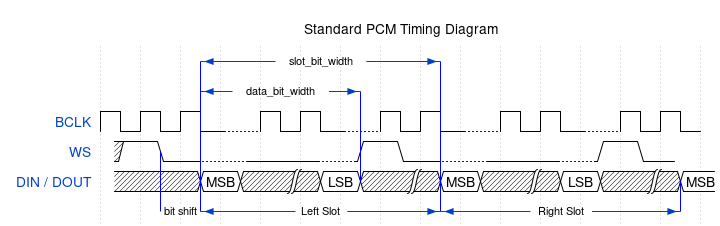
\includegraphics[width=0.7\linewidth]{Images/IS2PCM.png}
        \caption{Frame del bus I2S en mode d'operació justificat a la dreta. \cite{I2SESP32}}
        \label{I2SRightJust_fig}
    \end{figure}
    \item \textbf{Mode d'Operació Justificat a l'Esquerra:} A diferència del format justificat a la dreta, la configuració justificada a l'esquerra elimina qualsevol retard d'un cicle de rellotge relacionat amb BCLK. En aquesta configuració, ambdós canals tenen els seus bits més significatius (MSBs) validats a la primera vora ascendent de BCLK/SCK després de qualsevol modificació del WS. Això contrasta amb l'operació justificada a la dreta, ja que no requereix coneixement previ de la longitud de paraula abans d'iniciar la transmissió.
    \begin{figure}[H]
        \centering
        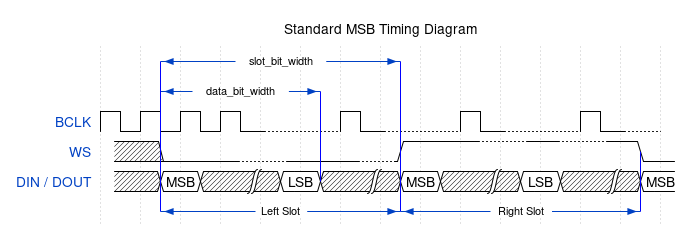
\includegraphics[width=0.7\linewidth]{Images/I2SMSB.png}
        \caption{Frame del bus I2S en mode d'operació justificat a l'esquerra. \cite{I2SESP32}}
        \label{I2SLeftJust_fig}
    \end{figure}
    \item \textbf{Mode d'Operació Estàndard Phillips:} Aquest estàndard es diferencia per un bit de rellotge respecte al format justificat a l'esquerra típic. En aquest cas, s'inicia la transmissió de dades pel Serial Data al segona flanc de pujada del Serial Clock un cop iniciada la transmissió per un canal diferent (canvi de nivell al Word Select).
    \begin{figure}[H]
        \centering
        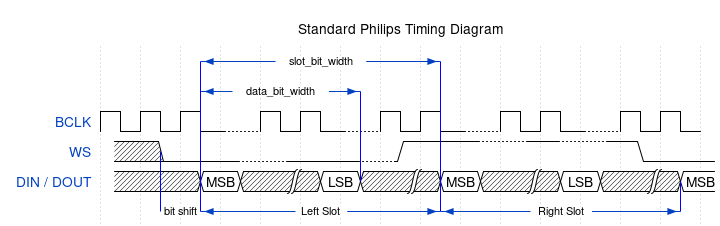
\includegraphics[width=0.7\linewidth]{Images/I2SPhilips.png}
        \caption{Frame del bus I2S en mode d'operació de l'estàndar Philips. \cite{I2SESP32}}
        \label{I2SPhilips_fig}
    \end{figure}
\end{itemize}
\par El Word Select indica el canal que s'està transmetent:
\begin{itemize}
    \item WS = 0: canal 1 (esquerra)
    \item WS = 1: canal 2 (dreta)
\end{itemize}

\par El senyal WS pot canviar tant en una vora descendent com en una vora ascendent del rellotge en sèrie, però no necessita ser simètric. En el dispositiu de destinació, aquest senyal es bloqueja en la vora ascendent del senyal de rellotge. La línia WS canvia un període de rellotge abans que es transmeti el MSB. Això permet que el transmissor de destinació estableixi una temporització síncrona de les dades sèrie que es configuraran per a la transmissió. A més, permet que el receptor emmagatzemi la paraula anterior i buidi l'entrada per a la següent paraula.

\section{Transformada de Fourier}
\par La transformada de Fourier descompon un senyal continu en el temps en un espectre de freqüència que defineix el senyal i per tant, redefineix el senyal en el domini freqüencial. La transformada de Fourier d'un senyal x(t) s'expressa de la següent manera \cite{Bose1985}:
\begin{equation}\label{eqTransFourier}
    X(w) = \int_{-\infty}^{+\infty} x(t)e^{-iwt} \,dt 
\end{equation}

\par I en temps discret, la transformada es redefineix de la següent manera\cite{ImmAudioSign}:
\begin{equation}\label{eqDiscreteFourier}
    X(w) = \sum_{k =-\infty}^{+\infty} x(k)e^{-iwk}
\end{equation}

\section{Teorema de Nyquist}
\par El teorema de Nyquist descriu com samplejar un senyal per evitar que no es perdi informació tot emprant la transformada de Fourier per a representar l'espectre en freqüència del senyal abans i després de ser mostrejada. El teorema diu així \cite{NYQUIST1928}:
\begin{quote}
    \textit{Donat un senyal continu en el temps x(t) limitada en l'ample de banda per fmax, estableix que per poder samplejar el senyal sense perdre informació, cal mostrejar-lo a una freqüència fsample $\geq$ 2fmax. Alternativament, es pot definir la frequencia de Nyquist com: \[f_{nyquist} = \frac{1}{2}f_{sample}\]}
\end{quote}
\par Teòricament, si a un senyal del món real s'aplica el teorema de Nyquist per mostrejar-lo en un sistema discret, és possible reconstruir el senyal original a partir de la freqüència de sampleig. En canvi, si un senyal conté freqüències més enllà de l'ample de banda considerat per al mostreig d'aquest senyal, el sistema resulta submostrejat i no serà possible reconstruir el senyal original. Per evitar situacions on la pèrdua sigui notòria i pugui perjudicar el processament d'aquests senyals, típicament els senyals es sobremostregen a freqüències més altes del doble de la freqüència mes alta en tot l'espectre del senyal a mostrejar.
\par No obstant, en la conversió dels senyals continus a temps discret, si s'omet part del seu espectre frequencial, dona lloc a l'efecte de l'aliàsing. Aquest efecte apareix com la superposició de les imatges a freqüències més altes del senyal sobre l'espectre mostrejat, entenent imatge com l'ample de banda del senyal que comprén: \[Nf_{sample} + 1 \leq f < (N+1)f_{sample}\] En el món pràctic, no existeixen senyals pures i la majoria tenen components de freqüència extremadament alta més enllà de la freqüència de Nyquist. 

\begin{figure}[H]
    \centering
    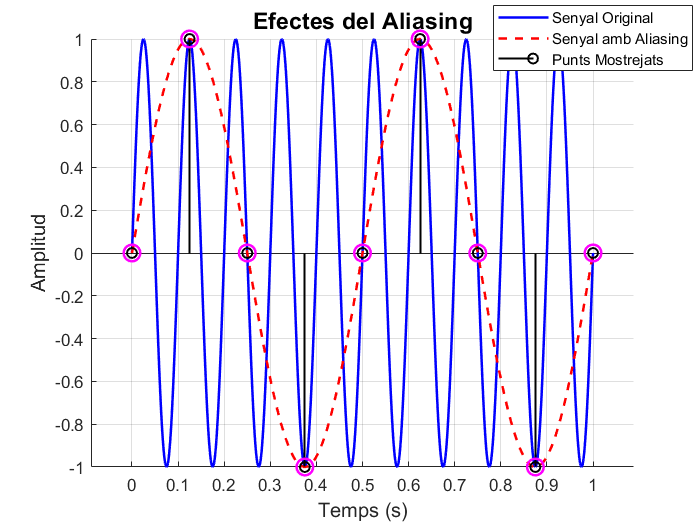
\includegraphics[width=0.5\linewidth]{Images/imatge_aliasing.png}
    \caption{Efectes de l'Aliasing en un senyal sinusoidal on la freqüència de mostreig es superior a la freqüència de Nyquist}
    \label{Aliasing_fig}
\end{figure}

\section{Transformada en \textit{z}}
\par La transformada en z es una generalització de la transformada de Fourier, que es pot expressar com les sèries de Laurent amb la variable complexa z = exp(jw). Donada una seqüència x[n], la corresponent transformada en z es defineix com\cite{ImmAudioSign}:
\begin{equation}\label{trans_z}
    X(z) =  \sum_{n=0}^\infty x(n)z^{-n}
\end{equation}
\par Un dels motius per utilitzar la transformada en z és que la transformada de Fourier no convergeix per tots els senyals en temps discret i és útil tenir una generalització de la transformada de Fourier que englobi una classe més àmplia de senyals.
\par Com es pot apreciar observant les equacions \ref{eqDiscreteFourier} i \ref{trans_z}, existeix una relació directa entre la transformada de Fourier i la transformada en \textit{z}. Aquesta relació es pot constatar substituint la variable z en l'equació \ref{trans_z} per la variable complexa exp(jw), aleshores la transformada en z es redueix a la transformada de Fourier. Aquest és un dels motius pels quals s'empra la notació de la transformada de Fourier en termes de exp(jw), doncs facilita el canvi de domini de temps discret a freqüencial \cite{DiscreteTimeSP}. Això es correspon a una restricció de la variable z amb magnitud unitària. De manera més genèrica és possible expressar la variable z en forma polar com: \[z = re^{jw}\] Amb aquesta última expressió de z, si es substitueix a \ref{trans_z} es converteix en l'equació \ref{eqDiscreteFourier}.

\par En el pla z, el contorn que es correspon amb abs(z) = 1 és un cercle de radi la unitat, també referit com el cercle unitari. La transformada en z estudiada dins d'aquest cercle es correspon a la transformada de Fourier. En el pla polar z, l'angle que forma el vector que apunta a un punt z dins el cercle unitari es correspon a la pulsació w en rad/s. I doncs, si s'evaluessin els punts en el cercle unitari per w = 0 a w = 2$\pi$, es correspondria a examinar la transformada de Fourier en l'espectre de freqüències de 0 a 2$\pi$. Aquesta interpretació equival conceptualment a embolicar l'eix de freqüència de la transformada de Fourier al voltant del cercle unitari.

\section{Processament Digital de Senyals}
\subsection{Senyals en temps discret}
\par Els senyals en temps discret es representen matemàticament com seqüències de números, on l'n-èssim número s'indica com x[n].
\par En els senyals de temps discret, els valors del senyal es representen en intèrvals discrets i com seqüències de números, on l'n-èssim número s'indica com x[n] o x[nTs]. Ts representa el període de mostreig i defineix l'interval de temps en que es prenen els valors d'un senyal continu. 
\par En l'estudi dels senyals i sistemes en temps discret, apareixen sovint un seguit de senyals que juguen un paper important. Aquestes són \cite{DiscreteTimeSP}:
\begin{itemize}
    \item impuls unitari: La sequència que defineix aquest senyal es caracteritza per ser 1 en n = 0 i 0 en qualsevol altre instant. 
    \begin{equation}\label{delta_unit}
        \delta(n) = \left\lbrace\begin{array}{c} 1\quad n = 0 \\ 0\quad n \neq 0 \end{array}\right.
    \end{equation}
    \begin{figure}[H]
        \centering
        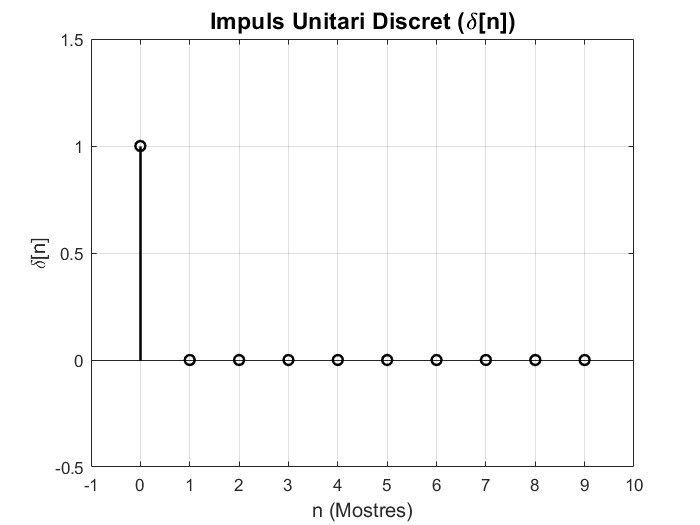
\includegraphics[width=0.5\linewidth]{Images/imatge_delta.png}
        \caption{Impuls unitari en temps discret de n = 10 mostres.}
        \label{delta_imp_fig}
    \end{figure}
    \item esglaó unitari: aquest senyal té valor zero pels instants abans de zero i pren valor unitari en l'instant zero i posteriors.
    \begin{equation}\label{step_unit}
        u(n) = \left\lbrace\begin{array}{c} 1\quad n \geq 0 \\ 0\quad n < 0 \end{array}\right.
    \end{equation}
    \begin{figure}[H]
        \centering
        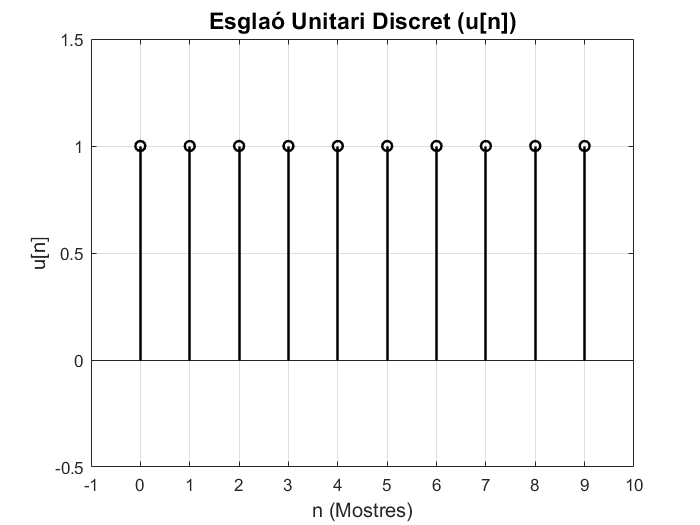
\includegraphics[width=0.5\linewidth]{Images/imatge_esglao.png}
        \caption{Esglaó unitari en temps discret de n = 10 mostres.}
        \label{step_fig}
    \end{figure}
    \item rampa discretitzada: per instants previs a zero pren valor zero, i a partir de l'instant zero pren el n-èssim valor que representa.
    \begin{equation}\label{ramp_func}
        u(n) = \left\lbrace\begin{array}{c} n\quad n \geq 0 \\ 0\quad n < 0 \end{array}\right.
    \end{equation}
    \begin{figure}[H]
        \centering
        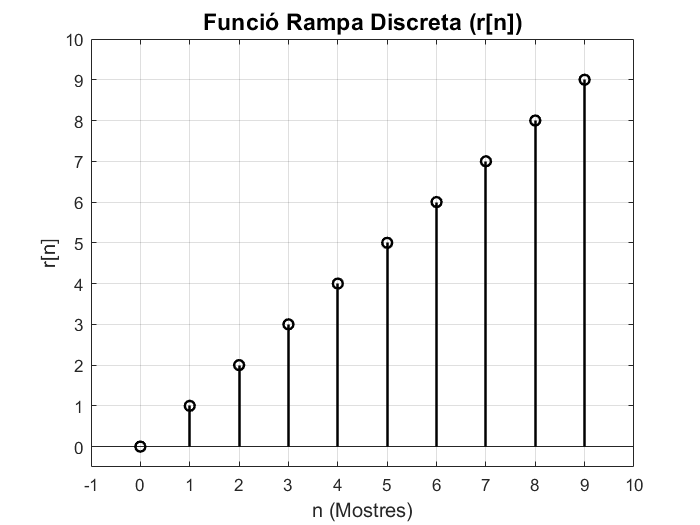
\includegraphics[width=0.5\linewidth]{Images/imatge_rampa.png}
        \caption{Funció rampa en temps discret de n = 10 mostres.}
        \label{ramp_fig}
    \end{figure}    
\end{itemize}

\par En el domini digital, els senyals només es poden representar en un rang de nombres enters i en la conversió de temps continu a temps discret és necessari aplicar un procés de requantificació. Aquesta transformació insereix soroll inevitablement al senyal, que mitjançant tècniques de processament digital és possible mitigar. Aquest soroll és complicat de descriure matemàticament doncs no és exactament lineal ni previsible en sistemes complexos de processament de senyals. No obstant, existeixen tècniques de modulació de soroll que mitiguen aquest fenomen d'acoplament de senyals indesitjat i que més endavant en aquest treball es comentaran breument.
\subsection{Sistemes en temps discret}
\subsubsection{Sistemes Lineals}
\par Les operacions realitzades per un sistema de processament digital es basen en la premissa que el sistema satisfà les propietats de linearitat i invariància en el temps. Si considerem un sistema lineal, les transformacions que aquest sistema realitza compleixen les propietats d'homogeneïtat, additivitat i de superposició \cite{DiscreteTimeSP}. A continuació es poden observar les demostracions:
\begin{itemize}
    \item Additivitat: Donat un sistema \textit{S} que a una entrada $x_1$ obté a la sortida $y_1$ i que a una entrada $x_2$ respon amb $y_2$, el sistema compleix la propietat d'additivitat si es satisfà:
    \begin{equation}\label{additivity_eq}
        S(x_1 + x_2) = y_1 + y_2
    \end{equation}
    \item Homogeneitat: Donat un sistema \textit{S} que a una entrada $x_1$ obté a la sortida $y_1$, el sistema compleix la propietat d'homogeneitat si es satisfà:
    \begin{equation}\label{homogeneity_eq}
        S(ax_1) = ay_1
    \end{equation}
    \item Superposició: Si un sistema \textit{S} es considera lineal i compleix les propietats d'homogeneitat i linealitat, per necessitat compleix la propietat de superposició. La demostració de la propietat de superposició d'un sistema \textit{S}, s'expressa de la següent forma:
    \begin{equation}
        S(ax_1+ax_2) = ay_1 + ay_2
    \end{equation}
\end{itemize}


\subsubsection{Sistemes de Temps Invariant}
\par  Un sistema invariant en el temps és aquell per al qual una entrada retardada de n mostres resulta en una sortida retardada de n mostres. Específicament, si considerem un sistema \textit{S}, per una entrada retardada k mostres es considera que el sistema és invariant en el temps si:  
\begin{equation}
    S(x(n-k)) = y(n-k)
\end{equation}

\subsubsection{Sistemes de Temps Invariant i Lineals}
\par Els sistemes lineals i de temps invariant tenen aplicacions rellevants en el processament digital de senyals degut que les propietats d'aquests sistemes estan definides per les de la convolució en temps discret. 

\par Aquests sistemes tenen la propietat que essent y(n) la resposta a la seqüència d'entrada x(n), la resposta a la seqüència desplaçada x(n-k) és y(n-k), que és la mateixa resposta que a la seqüència x(n), desplaçada per la mateixa quantitat k. A causa d'aquesta propietat, es pot demostrar immediatament que si un sistema és lineal i invariant en el temps, es pot caracteritzar per la seva resposta a un impuls unitari. Per als sistemes lineals invariants en el temps, l'expressió genèrica que els defineix ve donada per:
\begin{equation}\label{eq_summ_lti}
    y[n] = \sum_{k=-\infty}^{\infty} x[k]h_k[n] 
\end{equation}
\par L'equació \ref{eq_summ_lti} també es coneix com convolució i demostra que un cop es coneix h(n), és possible determinar la resposta a qualsevol altra seqüència d'entrada x(n). \cite{DiscreteTimeSP} 

\section{Filtres Digitals}
\subsection{Filtres FIR}
\par De la traducció literal de la seva denominació anglosaxona, els filtres FIR són filtres amb una \textit{Resposta d'Impuls Finit}, altrament referits com filtres de mitjana mòbil, filtres transversals o, en referència a la naturalesa de la seva implementació, filtres no recursius. En el processament digital de senyals d'àudio, són la topologia de filtres més populars degut a la baixa complexitat en la implementació i la linealitat en la seva resposta en fase.
\par Els filtres FIR posseeixen certes característiques desitjables, per definició són sistemes de tipus Lineal i Invariant al Temps és a dir, com s'ha comentat a l'apartat de sistemes Lineals i de Temps Invariant, compleixen les propietats de superposició, homogeneïtat i invariança. Conseqüentment, tenen un seguit de ventatges en l'espectre freqüencial com el desfassament lineal, l'estabilitat inherent i la baixa sensibilitat als errors de quantificació \cite{DigitalSignalPr}. La resposta d'un filtre de longitud L o ordre N = L - 1, ve donada per la convolució de les mostres actuals i anteriors a l'entrada del filtre, i els coeficients del mateix. I la funció de transferència en el domini \textit{z} ve definida per:
\begin{equation}\label{eq_FIR}
    H(z) = \sum_{k=-\infty}^{\infty} h_k z^{-n}
\end{equation}
\par Els coeficients $h_k$ defineixen els zeros del filtre caracteritzant la resposta en freqüència. La presència de només zeros al polinomi \ref{eq_FIR} confirma la teòrica estabilitat dels filtres FIR.
\begin{figure}[H]
    \centering
    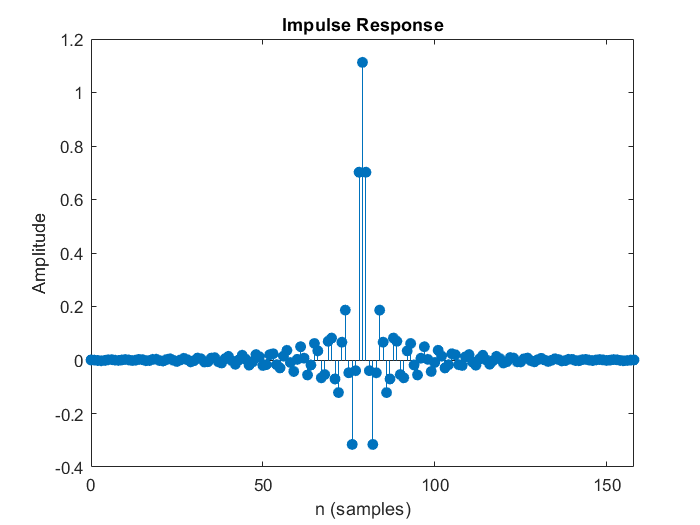
\includegraphics[width=0.5\linewidth]{Images/FIRimpulse.png}
    \caption{Resposta a un impuls unitari d'un filtre FIR}
    \label{figFIRimpulse}
\end{figure}

\subsubsection{Filtres CIC}
\par En el processament de senyals digitals, un Cascaded Integrator-Comb (CIC) és una classe computacionalment eficient de filtres FIR passa-baixos, que encadena N nombre de parells integradors i filtres de pinta (on N és l'ordre del filtre) per formar un decimador o interpolador. Els filtres de pinta són blocs que s'utilitzen en el processament digital de senyals en realitzar la suma d'una mostra retardada amb l'actual \cite{CICLyons}. 
\begin{figure}[H]
    \centering
    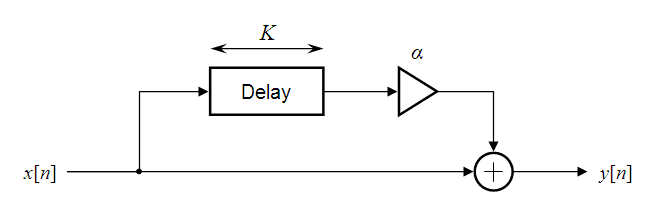
\includegraphics[width=0.5\linewidth]{Images/Comb_filter_feedforward.png}
    \caption{Bloc de filtrat Comb o de pinta. \cite{CICLyons}}
    \label{figComb}
\end{figure}
\par Els filtres CIC s'originen a partir de la reestructuració dels interpoladors de mitjana mòbil com el de la figura \ref{figMAFilter}. A partir de la equació \ref{eqMovAv}, es pot intuir que els blocs CIC mantenen la propietat d'interpolació amb l'afegit que la resposta en freqüència es veu modificada per la presència dels blocs integradors i Comb. Més específicament, modificant els blocs Comb es situen els zeros i amb els blocs integradors els pols de la funció de trasferència. 
\begin{figure}[H]
    \centering
    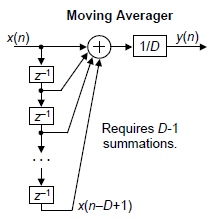
\includegraphics[width=0.3\linewidth]{Images/fir-mvavg-form.png}
    \caption{Diagrama de blocs d'un filtre de mitjana mòbil.}
    \label{figMAFilter}
\end{figure}

\begin{equation}\label{eqMovAv}
    y[n] = x[n] + x[n-1] + x[n-2] + x[n-3] \longrightarrow y[n] = y[n-1] + x[n] + x[n-4]
\end{equation}

\par En un CIC de delmat, el senyal d'entrada passa primer per N etapes integradores, seguides d'un procés de mostreig descendent, i finalment per N etapes de diferència (etapes de Comb). D'altra banda, un CIC interpolador segueix l'ordre invers d'aquesta arquitectura: primer aplica N etapes de Combs, seguit del zero stuffing i, finalment, N etapes integradores \cite{Hogenauer1981}.
\begin{figure}[H]
    \centering
    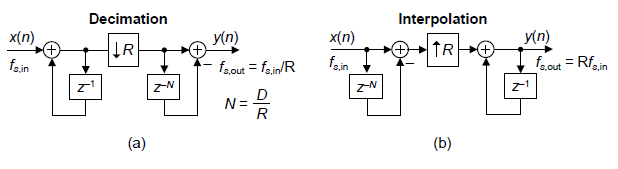
\includegraphics[width=0.7\linewidth]{Images/CIC_digital_filters.png}
    \caption{Implementacions de filtres CIC en una sola etapa: (a) Delmat; (b) Interpolació \cite{CICLyons}}
    \label{figCICDeciInt}
\end{figure}
\newpage
\subsection{Filtres IIR}
\par La resposta a un impuls unitari d'aquests filtres és una seqüència infinita, fet que dona lloc a la seva denominació com a filtres IIR (\textit{Infinite Impulse Response}). Típicament, aquests filtres requereixen menys recursos i poden executar tasques de filtratge a major velocitat que els filtres FIR. 
\par En un filtre IIR implementat de manera recursiva, la mostra de sortida y(k) és una combinació lineal de les mostres d’entrada actuals i passades de la seqüència x(k), així com de les mostres de sortida passades. Aquesta estructura recursiva és la clau per obtenir una alta eficiència i permet que els filtres IIR es comportin com una aproximació dels sistemes analògics \cite{Bose1985}.
\par Un filtre IIR no és útil si no és estable. Per tant, cal fer comprovacions d'estabilitat en tots els dissenys, i si es detecta que un filtre és inestable, s’han de proporcionar esquemes satisfactoris d'estabilització. En moltes aplicacions, on es busca la linealitat de la característica de fase com en el tractament de senyals d'àudio, un filtre IIR sol ser poc pràctic\cite{DigitalSignalPr}.
\par Comparat amb un filtre FIR, un filtre IIR sovint pot ser molt més eficient en termes d'assolir certes característiques de rendiment amb un ordre de filtre determinat. Això es deu al fet que el filtre IIR incorpora retroalimentació i és capaç de realitzar tant els zeros com els pols d'una funció de transferència del sistema, mentre que el filtre FIR és un filtre només de zeros. Però, per contrapartida, els filtres IIR són més sensibles a la quantificació dels coeficients i poden derivar en inestables si la requantificació no es fa correctament. A l'equació \ref{eqIIR} s'expressa la funció de transferència general dels filtres IIR.
\begin{equation}\label{eqIIR}
    H_{IIR}(z) = \frac{\sum_{k=0}^{M} b_k z^{-k}}{\sum_{k=0}^{M} a_k z^{-k}}
\end{equation}

\section{Modulador $\Sigma \Delta$}
\par Els moduladors $\Sigma \Delta$ o $\Delta \Sigma$ son una topologia de convertidors ADC o DAC molt popular per la seva propietat de modelat del soroll de quantificació. 
\par La tècnica de modulació sigma-delta és la tecnologia més popular en convertidors d'àudio A/D i D/A dels últims 30 anys, gràcies al modelat de soroll característic de la seva estructura. La nomenclatura utilitzada per descriure aquest tipus de modulació reflecteix les seves propietats tècniques i explica per què és especialment atractiva per a la implementació en convertidors tant A/D com D/A.
\par La lletra $\Delta$ prové de l'alfabet grec i, en el context matemàtic, s'utilitza habitualment per representar variacions o diferències d'una magnitud. En la tècnica de modulació sigma-delta, $\Delta$ fa referència al càlcul de la diferència entre la mostra d'entrada i la sortida anterior quantitzada.

\par D'altra banda, la lletra $\Sigma$, també originària de l'alfabet grec, s'empra sovint per representar processos de suma. En el cas del modulador en qüestió, aquesta suma correspon a una integral en temps discret. L'efecte d'aquest bloc integrador és el que fa que la tècnica de modulació sigma-delta sigui tan interessant per a aplicacions amb requeriments exigents pel que fa al SNR del senyal. Aquest bloc es tractarà amb més detall més endavant. 
\par Essencialment, un convertidor $\Sigma \Delta$ digitalitza el senyal d'entrada amb baixa resolució (típicament d'1 bit però es poden implementar estructures amb més nivells segons el quantificador a la sortida) a una freqüència de mostreig alta. L'efecte del sobremostreig distribueix el soroll de quantificació en un espectre de freqüència més ampli que el del senyal d'interès. L'altre fenomen interessant del modulador és l'atenuació del soroll de quantificació, ja que el bloc es comporta com un filtre passa-alts per l'error en el procés de quantificació, provocant que la major part de la potència del soroll no desitjat es situï més enllà de l'amplada de banda del senyal d'interès. Per tant, en el modulador $\Sigma \Delta$ l'efecte del sobremostreig juntament amb la modulació del soroll de quantificació permeten millorar el SNR del senyal d'entrada i obtenir alts rendiments a baix cost computacional. Addicionalment, el senyal que conté la informació d'interès no es veu modificat. 
\par L'estructura més bàsica de les topologies $\Sigma \Delta$ permet entendre les propietats dels moduladors derivats d'aquesta família. A partir del sistema representat a la figura \ref{figMOD1}, que mostra un modulador $\Sigma \Delta$ de primer ordre amb realimentació negativa, es pot descriure el seu comportament mitjançant l'equació \ref{eqMOD1}.
\begin{figure}[H]
    \centering
    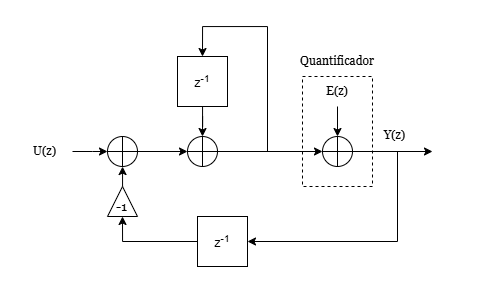
\includegraphics[width=0.5\linewidth]{Images/SigmaDeltaMOD1.drawio.png}
    \caption{Modulador $\Sigma \Delta$ de primer ordre.}
    \label{figMOD1}
\end{figure}
\begin{equation}\label{eqMOD1}
    Y(z) = 1 \ U(z) + (1 - z^{-1})E(z)
\end{equation}
\par A partir de l'equació \ref{eqMOD1}, es pot observar que el senyal d'entrada U(z) no es veu afectada pel sistema implementat, mentre l'error de quantificació està modelat per un filtre passa alts de primer ordre (1 - $z^{-1}$). A la figura \ref{fig_NTFpendent} es pot apreciar el comportament del modelat del soroll de quantificació del sistema, amb una pendent de la banda de transició de 20 dB/dec. 
\begin{figure}[H]
    \centering
    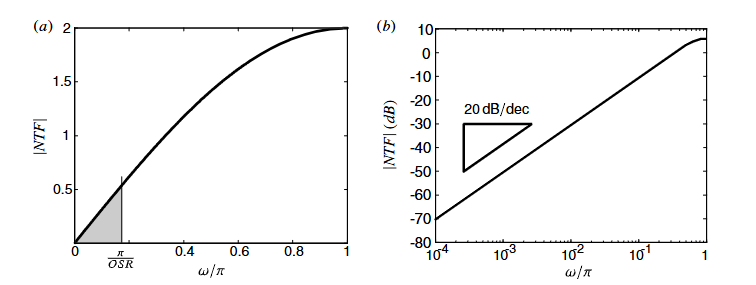
\includegraphics[width=0.6\linewidth]{Images/graficaNTFMOD1.png}
    \caption{Resposta en freqüència de NTF(z) d'un modulador $\Sigma \Delta$ de primer ordre. \cite{UndrstndSDM}}
    \label{fig_NTFpendent}
\end{figure}

\par L'ús d'integradors permet que la funció de transferència del senyal (STF) mantingui un guany unitari, mentre que el soroll de quantificació es redueix significativament a la banda de freqüència d'interès. Aquest enfocament permet aconseguir un SNR o SNDR més elevat segons els requisits del sistema. No obstant, l'addició de més etapes integradores no es pot fer manera directa ja que presenta problemes d'estabilitat. Degut a que cada etapa afegeix un canvi de fase de 90º, l'ordre del filtre de retroalimentació no pot ser més gran de 2. 

\subsubsection{Topologies de moduladors $\Sigma \Delta$}
\par A banda de l'estructura fonamental dels moduladors $\Sigma \Delta$ com el de la figura \ref{figMOD1}, existeixen diverses topologies que s'han desarollat per poder afrontar requeriments més exigents que els assumibles per un modulador de primer ordre. A continuació es comentaran breument les més rellevants \cite{SDMToolbox}:
\begin{itemize}
    \item \textbf{CIFB}: Els coeficients $a_n$ ubiquen els pols del NTF i el STF, mentre que els coeficients $b_n$ mapejen els zeros del STF. Els coeficients de les variables d'estat $c_n$ s'utilitzen per escalar el rang dinàmic.
    \begin{figure}[H]
        \centering
        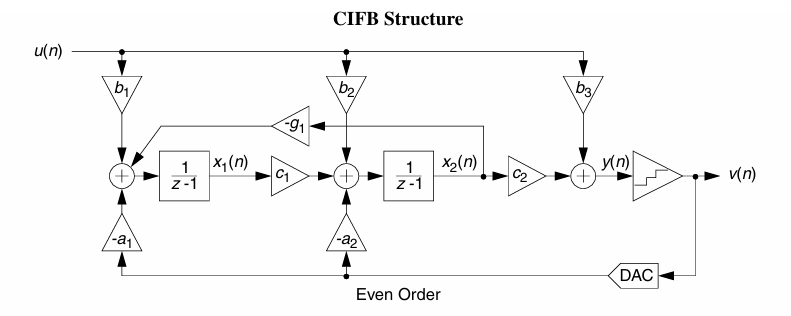
\includegraphics[width=0.5\linewidth]{Images/CIFB.png}
        \caption{Modulador $\Sigma \Delta$ CIFB}
        \label{figCIFB}
    \end{figure}
    \item \textbf{CRFB}: L'estructura és similar als CIFB a diferència del ressonador estable que es forma amb la implementació d'un bloc integrador amb delay i un bloc integrador sense i el llaç de realimentació creat amb $g_n$.
    \begin{figure}[H]
        \centering
        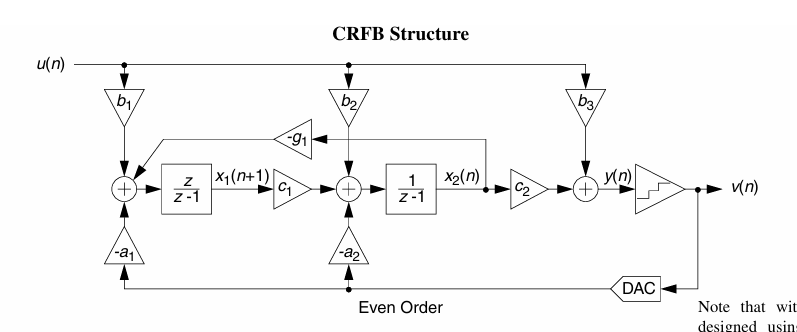
\includegraphics[width=0.5\linewidth]{Images/CRFB.png}
        \caption{Modulador $\Sigma \Delta$ CRFB}
        \label{figCRFB}
    \end{figure}
    \item \textbf{CIFF}: A la sortida es calcula la suma de les variables d'estat. El llaç de realimentació mitiga el soroll de quantificació.
    \begin{figure}[H]
        \centering
        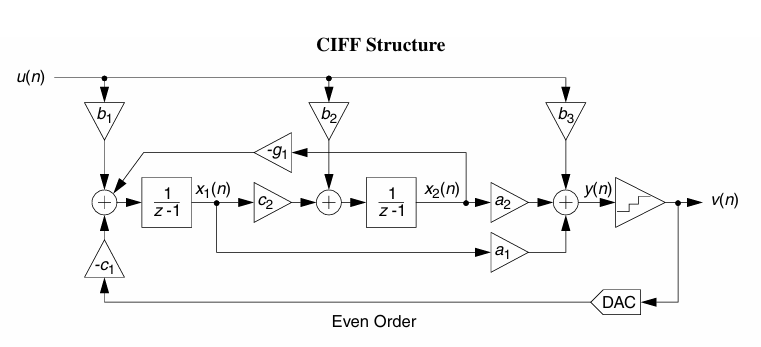
\includegraphics[width=0.5\linewidth]{Images/CIFF.png}
        \caption{Modulador $\Sigma \Delta$ CIFF}
        \label{figCIFF}
    \end{figure}
    \item \textbf{CRFF}: S'implementa l'estructura CIFF amb resonadors que afegeixen zeros complexes en NTF.
    \begin{figure}[H]
        \centering
        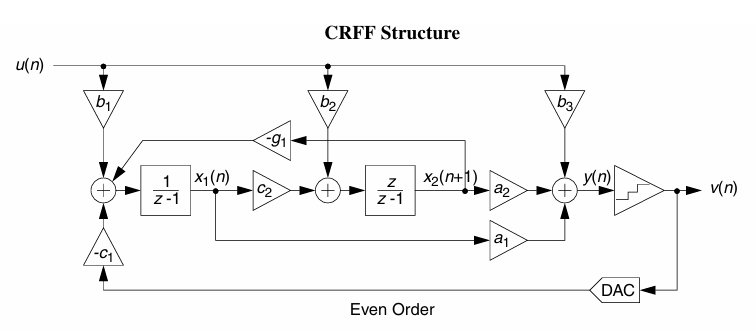
\includegraphics[width=0.5\linewidth]{Images/CRFF.png}
        \caption{Modulador $\Sigma \Delta$ CRFF}
        \label{figCRFF}
    \end{figure}
\end{itemize}
\section{PWM}
\par La modulació per amplada de pols (PWM) és una tècnica de control utilitzada en convertidors d'electrònica de potència per regular l'alimentació subministrada des de la font d'alimentació fins a la càrrega. En un senyal PWM, la freqüència del cicle de generació de polsos és un paràmetre fix i l'amplitud d'aquests polsos, una variable. D'aquesta forma, modificant l'amplitud dels polsos s'obté el valor promig a la càrrega equivalent al senyal original sense modular. Aquesta generació del senyal PWM es pot fer en domini analògic o en domini digital. En el domini analògic, els circuits amb amplificadors operacionals s'utilitzen àmpliament per generar PWM a partir de senyals portadores i modulants. Però aquests circuits són més susceptibles a les derives de la temperatura i a la degradació amb el pas del temps dels components que en conjunt acaben oferint un rendiment pitjor del sistema original. En el medi analògic, les entrades del modulador d'ample de banda són el senyal analògic a modular i una ona triangular com a tensió de referència per calcular l'amplitud dels polsos a la sortida. Anàlogament, en el medi digital s'aconsegueix un efecte similar i la implementació d'algorismes avançats és relativament fàcil i més ràpida. \cite{PWMarticle} 
\begin{figure}[H]
    \centering
    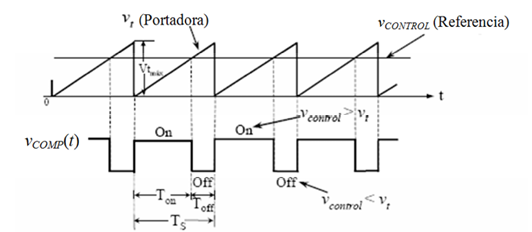
\includegraphics[width=0.5\linewidth]{Images/PWM_Pique.png}
    \caption{Frame dels senyals implicats en el procés de modulació per ample de polsos en el medi analògic, on el senyal de control representa l'amplitud a transmetre a la sortida. \cite{PiquePWR}}
    \label{PWM_analog_fig}
\end{figure}
\par Com es pot observar a la imatge \ref{PWM_analog_fig}, el temps que el senyal de sortida del modulador està a nivell alt és directament proporcional a la relació entre l'amplada del senyal de control i el del portador. Aquesta relació també es coneix com \textit{duty cycle} que es representa matemàticament de la següent forma:
\begin{equation}\label{duty_eq}
    \delta(t) = \frac{V_{control}(t)}{V_{t,max}(t)}
\end{equation}
On Vcontrol és el valor del senyal a modular i Emax, la tensió màxima del senyal triangular o portador.

\section{Mètriques de rendiment}

\subsection{SNR}
\par El Signal to Noise Ratio (SNR) ve donat per la relació entre la potència del senyal i la potència del soroll, per a una certa amplitud d'entrada. No té en compte els components del senyal harmònicament relacionats \cite{ADC16b}.
\begin{equation}\label{SNR_eq}
    SNR(dB) = 20log_{10}(\frac{P_{Senyal}}{P_{Soroll}})
\end{equation}
\par En el context del processament digital de senyals, sovint es menciona aquest mesura com SQNR (Signal to Quantization Noise Ratio) doncs en el domini digital es d'interès coneixer la capacitat d'un procés de mitigar el soroll provocat per la quantificació del senyal mostrejat. De \cite{UndrstndSDM}, s'obté que l'expressió del SQNR(dB) és:
\begin{equation}\label{eq_SQNR}
    SQNR(dB) = 10log_{10}(\frac{15 M^2 (OSR)^5}{2\pi^4})    
\end{equation}
on M és els nombre de nivells del quantificador.
\par De forma similar, el Signal to Noise and Distortion Ratio (SNDR) és la relació entre la potència del senyal i el soroll i tots els components de potència de distorsió. Així, té en compte diversos dels harmònics (típicament el 2n i el 3r harmònic) que es troben dins de la banda d'interès. \cite{SDMClassD}

\subsection{DR}
\par El Dynamic Ratio (DR) és el rang d'amplituds del senyal sobre el qual l'estructura funciona correctament, és a dir, dins dels límits acceptables de distorsió. Està determinat pel senyal d'entrada d'amplitud màxima i pel senyal d'entrada detectable més petit. \cite{ADC16b}
\begin{equation}
    DR(dB) = 10log_10(\frac{3(2^{B}-1)^{2}(2L+1)OSR^{2L +1}}{2\pi^{2L}}
\end{equation}

\subsection{THD}
\par La distorsió harmònica total és la relació entre la suma de la potència del senyal de totes les freqüències harmòniques per sobre de la freqüència fonamental i la potència de la freqüència fonamental. La distorsió harmònica generada per un n-èsim harmònic específic també es pot determinar i està donada per la relació entre la potència del senyal i la potència del component de distorsió en aquest n-èsim harmònic de la freqüència del senyal \cite{PiquePWR}.
\begin{equation}
    THD = \frac{\sqrt{V_{n+1}^{2}+V_{n+2}^{2}+V_{n+3}^{2}+...}}{V_{n}^{2}}
\end{equation}

\subsection{Soroll de Quantificació}
\par El procés de quantificació inevitablement introdueix distorsió en la senyal degut a que en la conversió d'un senyal continu al domini digital es perd informació. Aquest procés té una característica d'escala i la diferència entre dos valors quantificats adjacents s'anomena mida de pas ($\Delta$). Per a valors d'entrada grans, la sortida del quantificador pot arribar a saturar. L'interval de conversió pel qual el quantificador no desborda, s'anomena interval d'escala completa (FS) del quantitzador. Un quantitzador amb un nombre de bits N, pot representar fins a 2N nivells d'amplitud, donant com a resultat un $\Delta$ donat per:
\begin{equation}\label{eq_stepsize}
    \Delta = \frac{FS}{N}
\end{equation}
\par En el procés de quantificació, totes les entrades s'arrodoneixen al nivell més pròxim fet que implica que l'error induït pel procés es troba en el rang [$-\frac{\Delta}{2}$, $\frac{\Delta}{2}$]. Si es considera que la distribució d'aquest error és uniforme en tot el rang d'aparició, la potència mitjana és:
\begin{equation}\label{eq_pwrquant}
    P_{q_{e}}\ = \frac{1}{\Delta} \int_{-\frac{\Delta}{2}}^{\frac{\Delta}{2}} q_{e}^2 \ d q_{e} = \frac{\Delta^2}{12}
\end{equation}
\par Com més gran sigui la resolució del quantificador, més petit és $\Delta$. Així, augmentant el nombre de bits (N) del quantitzador, la potència mitjana del soroll disminueix. 
\par Quan es mostreja un senyal a una freqüència $f_s$, la distribució del soroll de quantificació és uniforme al llarg del rang de freqüències [$-\frac{f_s}{2}$, $\frac{f_s}{2}$]. Per tant, la distribució de la potència del soroll espectral ve donada per: 
\begin{equation}\label{eq_energy_quant}
    E(f) = \frac{\Delta^2}{12 f_s}
\end{equation}
\par De l'equació \ref{eq_energy_quant} es dedueix que, amb una major freqüència de mostreig, l'error de quantificació es redistribueix en un espectre més ampli, reduint així la densitat espectral d'aquest error. Per tant, el procés de sobremostreig contribueix a disminuir l'impacte de l'error de quantificació en la banda de freqüències d'interès.
